\section{Theoretische Grundlagen}

\subsection{Spin-$\frac{1}{2}$-Teilchen im konstanten Magnetfeld}
Teilchen mit Spin $\vec{S}$ und gyromagnetischem Verhältnis $\gamma$ haben ein magnetisches Moment
\begin{align*}
  \vec{\mu}=\gamma\vec{S}.
\end{align*}
In einem Magnetfeld $\vec{B}$ ist der Hamiltonoperator (für die Spinwellenfunktion) also gegeben durch
\begin{align}
  H=-\vec{\mu} \cdot \vec{B}=-\gamma \vec{B} \cdot \vec{S} \label{hamilton1}
\end{align}

Für eine anschauliche Beschreibung wird der Bloch-Vektor durch die Erwartungswerte der Pauli-Matrizen definiert:
\begin{align*}
  \vec{K}= \left( \begin{array}{c}
                    \braket{\sigma_x} \\
                    \braket{\sigma_y}\\
                    \braket{\sigma_z}
                  \end{array} \right).
\end{align*}
Aus dem Ehrenfest-Theorem und der Kommutatorrelation für Pauli-Matrizen folgt aus (\ref{hamilton1})
\begin{align}
  \diff{\vec{K}}{t}=\gamma \vec{K} \times \vec{B}.
\end{align}
Die (mittlere) Magnetisierung präzediert also um $\vec{B}.$ \\ \\

Im Folgenden wird die $z$-Achse als Quantisierungsachse gewählt, es soll also $\vec{B}=B\vec{e}_z$ gelten. Für Spin-$\frac{1}{2}$-Teilchen gibt es nur zwei mögliche Eigenwerte $m_z$ von $\vec{S}_z/\hbar$:
\begin{align*}
  m_z=\pm \frac{1}{2}.
\end{align*}
Es handelt sich also wie in Abbildung \ref{aufspaltung} zu sehen um ein zwei-Niveau-System.

\begin{figure}[h]
  \centering
  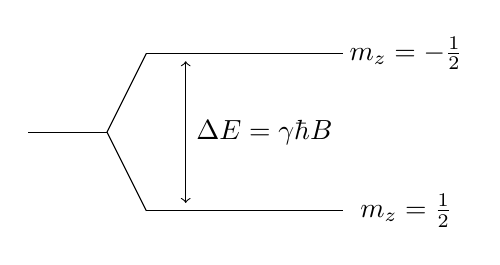
\begin{tikzpicture}
    \draw (0,0)--(1,0);
    \draw (1,0)--(1.5,1);
    \draw (1,0)--(1.5,-1);
    \draw (1.5,1)--(4,1);
    \draw (1.5,-1)--(4,-1);
    \draw [<->] (2,0.9)--(2,-0.9);
    \draw (3,0) node {$\Delta E=\gamma\hbar B$};
    \draw (4.8,1) node {$m_z=-\frac{1}{2}$};
    \draw (4.8,-1) node {$m_z=\frac{1}{2}$};
  \end{tikzpicture}
  \caption{Aufspaltung des Energieniveaus durch äußeres Magnetfeld}
  \label{aufspaltung}
\end{figure}

Wird nun eine Probe aus $N$ Teilchen in das Magnetfeld gebracht, so folgt beim thermischen Gleichgewicht aus der Boltzmann-Verteilung
\begin{align*}
  \frac{N_2}{N_1}=\exp \left( -\frac{\Delta E}{k_\mathrm{B}T} \right),
\end{align*}
wobei $N_1$ ($N_2$) die Besetzungszahl des energetisch niedrigeren (höheren) Zustandes, $k_\mathrm{B}$ die Boltzmann-Konstante und $T$ die Temperatur ist. Die gesamte Magnetisierung in $z$-Richtung ist gegeben durch 
\begin{align*}
  M_z=(N_1-N_2)\mu
\end{align*} 
mit $\mu=\gamma\hbar/2$, im thermischen Gleichgewicht gilt also
\begin{align*}
  M_z=M_0=N\mu\tanh \left(  \frac{\mu B}{k_\mathrm{B}T}\right).
\end{align*}

Bei ausgeschaltetem Magnetfeld ist die Probe zu Beginn unpolarisiert, es gilt also $M_z=0$. Nach \cite{manual} wird der Polarisationsvorgang nach Anschalten des Magnetfeldes durch 
\begin{align*}
  \diff{M_z}{t}=\frac{M_0-M_z}{T_1}
\end{align*}
beschrieben, wobei $T_1$ die materialabhängige longitudinale Relaxationszeit ist. Die Lösung der Differentialgleichung mit der Anfangsbedingung $M_z(0)=0$ ist
\begin{align}
  M_z(t)=M_0\left( 1-e^{-t/T_1} \right).
\end{align}
Mit der Anfangsbedingung $M_z(0)=-M_0$ bekommt die Exponentialfunktion in der Lösung einen zusätzlichen Faktor 2.

\subsection{Spin-$\frac{1}{2}$-Teilchen im magnetischen Wechselfeld}
Nun wird die Dynamik des Spins unter Einfluss eines zeitabhängigen magnetischen Feldes untersucht. Dazu wird das Feld 
\begin{align*}
  \vec{B}(t)= \left( \begin{array}{c}
                    B_1\cos\omega t\\
                    B_1\sin \omega t \\
                    B_0
                  \end{array} \right)
\end{align*}
betrachtet. Die resultierende Schrödingergleichung
\begin{align}
i\hbar \diff{}{t} \ket{\psi}=H(t)\ket{\psi} \label{hamilton2}
\end{align}
ist nicht mehr trivial lösbar. Um (\ref{hamilton2}) zu vereinfachen wird das Problem in einem mit $\vec{B}$ rotierenden Bezugssystem betrachtet:
\begin{align*}
  \ket{\psi} \rightarrow \ket{\tilde{\psi}}=\exp \left(  i\omega t \vec{S}_z/\hbar\right) \ket{\psi}.
\end{align*}
Für die transformierten Zustände folgt aus (\ref{hamilton2}) die Gleichung
\begin{align*}
  i\hbar \diff{}{t}\ket{\tilde{\psi}}= -\gamma \vec{B}_\mathrm{eff} \cdot \vec{S} \ket{\tilde{\psi}}
\end{align*}
mit dem effektiven Magnetfeld 
\begin{align*}
  \vec{B}_\mathrm{eff}=\left( \begin{array}{c}
                    B_1\\
                    0\\
                    B_0+\omega/\gamma
                  \end{array} \right).
\end{align*}
Im rotierenden Bezugssystem präzidiert die (mittlere) Magnetisierung also um $\vec{B}_\mathrm{eff}$. \\ \\
Für den Fall, dass $B_0=-\omega/\gamma$ gilt, rotiert die Magnetisierung im rotierenden Bezugssystem um die $x$-Achse. Wird das Magnetfeld z.B. für eine Dauer von $t=\pi/(2\gamma B_1)$ eingeschaltet, kann eine anfängliche Magnetisierung in $z$-Richtung in die $x$-$y$-Ebene gedreht werden ($\pi/2$-Puls). Der $\pi/2$-Puls ist elementar für den Versuch, da mit dem Aufbau nur die Magnetisierung in der $x$-$y$-Ebene gemessen werden kann. \\ \\
Wird ein $\pi/2$-Puls auf eine in $z$-Richtung polarisierte Probe angewendet, wird die Gesamtmagnetisierung in der $x$-$y$-Ebene aufgrund von Wechselwirkungen der Teilchen untereinander exponentiell abfallen (siehe \cite{manual}). Mit der dafür charakteristischen Zeit, der transversalen Relaxationszeit $T_2$, gilt also
\begin{align}
  M_{x/y}(t)=M_{x/y}(0) e^{-t/T_2}.
\end{align}
Dieses abnehmende Signal welches auf dem Oszilloskop sichtbar wird nennt sich FID (free induction decay).

\subsection{Hahn-Spinecho-Sequenz}
In der Praxis ist das Magnetfeld im Bereich der Probe nicht homogen. Das führt nach \cite{wikinmr} dazu, dass die effektive transversale Relaxationszeit durch
\begin{align*}
  \frac{1}{T_2^*}=\frac{1}{T_{2,\mathrm{inhom}}}+\frac{1}{T_2}
\end{align*}
gegeben ist. $T_{2,\mathrm{inhom}}$ ist dabei vom Magnetfeld abhängig. \\ \\
Die Hahn-Spinecho-Sequenz erlaubt die Messung von $T_2$. Dazu wird nach einem $\pi/2$-Puls und einer Wartezeit $\tau$ ein $\pi$-Puls auf die Probe gegeben. Nach einer weiteren Wartezeit $\tau$ erreicht die Magnetisierung ein Maximum welches unabhängig von $T_{2,\mathrm{inhom}}$ ist. Das Zustandekommen lässt sich gut an Abbildung \ref{hahn} nachvollziehen. Wenn das Magnetfeld $B_1$ örtlich schwankt präzedieren die Magnetisierungen an verschiedenen Orten etwas langsamer bzw. schneller als das rotierende Bezugssystem. Durch den $\pi$-Puls laufen die Magnetisierungsvektoren anschließend wieder zusammen und sind so an einem Zeitpunkt wieder parallel. 

\begin{figure}[h]
  \centering
  \begin{tikzpicture}
    \coord{0}{0}
    \draw [->,line width=0.5mm](0,0)--(0,1.5);
    \draw [->] (3,1)--(4,1);
    \draw (3.5,1.3) node {$\pi/2$};
    \coord{5}{0}
    \draw [->,line width=0.5mm](5,0)--(6.5,0);
    \draw [->] (8,1)--(9,1);
    \draw (8.5,1.3) node {$\tau$};
    \coord{10}{0}
    \draw [->,line width=0.5mm](10,0)--(11,0.5);
    \draw [->,line width=0.5mm](10,0)--(11.1,-0.6);
    \draw [->] (11.3,0) arc (0:40:0.7);
    \draw [->] (11.3,0) arc (0:-40:0.7);
    \draw [->] (0,-3)--(1,-3);
    \draw (0.5,-2.7) node {$\pi$};
    \coord{2}{-4}
    \draw [->,line width=0.5mm](10-8,0-4)--(9-8,0.5-4);
    \draw [->,line width=0.5mm](10-8,0-4)--(8.9-8,-0.6-4);
    \draw [<-] (0.7,-3.95) arc (180:140:0.7);
    \draw [<-] (0.7,-4.05) arc (180:220:0.7);
    \draw [->] (5,-3)--(6,-3);
    \draw (5.5,-2.7) node {$\tau$};
    \coord{8}{-4}
    \draw [->, line width=0.5mm] (8,-4)--(6.5,-4);
  \end{tikzpicture}
  \caption{Hahn-Spinecho-Sequenz im rotierenden Bezugssystem, die Magnetisierung (fett eingezeichnet) präzediert abhängig vom Magnetfeld schneller bzw. langsamer.}
  \label{hahn}
\end{figure}

\subsection{Carr-Purcell- und Meiboom-Gill-Sequenz}
Mit der Carr-Purcell-Sequenz können im Gegensatz zur Hahn-Spinecho-Sequenz direkt mehrere Echos hintereinander gemessen werden. Die Puls-Sequenz liest sich
\begin{align*}
  \pi/2 \rightarrow \tau \rightarrow \pi \rightarrow \tau \rightarrow \pi \rightarrow ... 
\end{align*}
Die Echos haben also eine Periode von $2\tau$. \\ \\
Problematisch ist die Carr-Purcell Methode wenn die Pulse nicht exakt die gewollte Länge haben. Dann summiert sich der systematische Fehler nämlich auf. Vermeiden lässt sich dies durch das verwenden der Meiboom-Gill-Sequenz. Bei dieser alterniert das Vorzeichen der $\pi$-Pulse, die gesamte Sequenz liest sich also 
\begin{align*}
  \pi/2 \rightarrow \tau \rightarrow \pi \rightarrow \tau \rightarrow -\pi \rightarrow ... 
\end{align*}
